\begin{appendices}
\chapter{Pielikums}
\label{appx:riceplots}

\begin{figure}[H]%!ht
	\centering
	\captionsetup{justification=centering}
	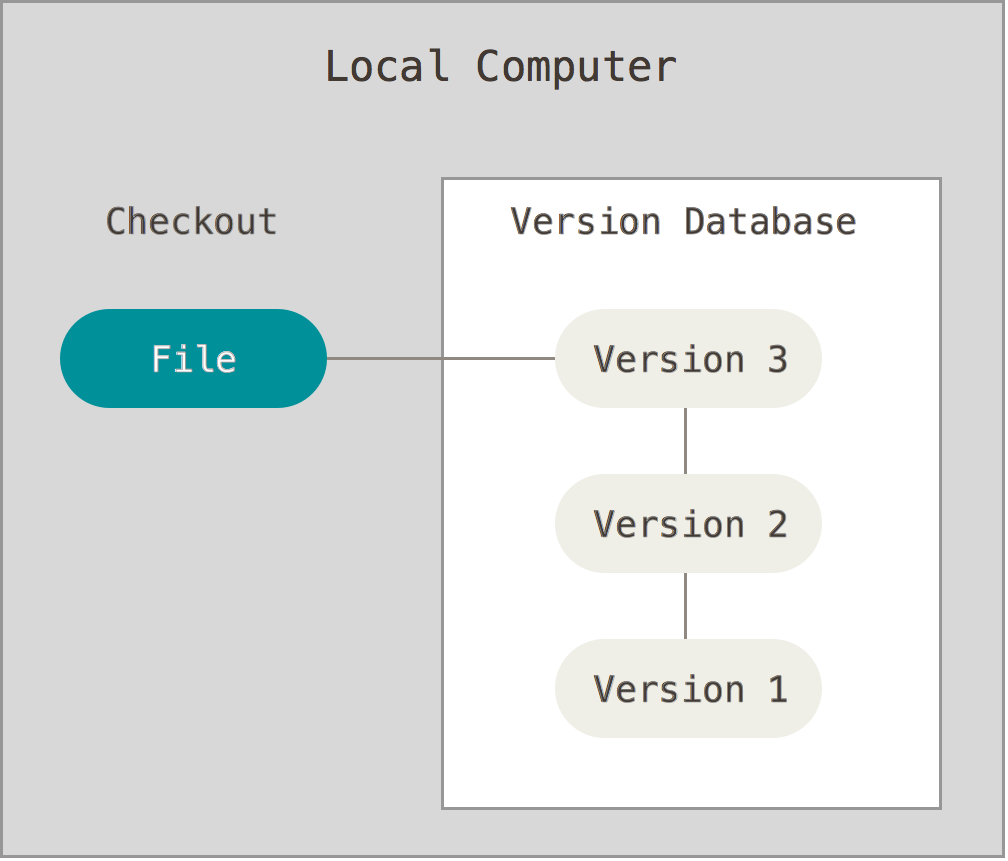
\includegraphics[width=0.8\textwidth]{VersionControlLocal.png}
	\caption{Lokālas VCS}
	\label{appfig:VersionControlLocal}
\end{figure}

\begin{figure}[H]%!ht
	\centering
	\captionsetup{justification=centering}
	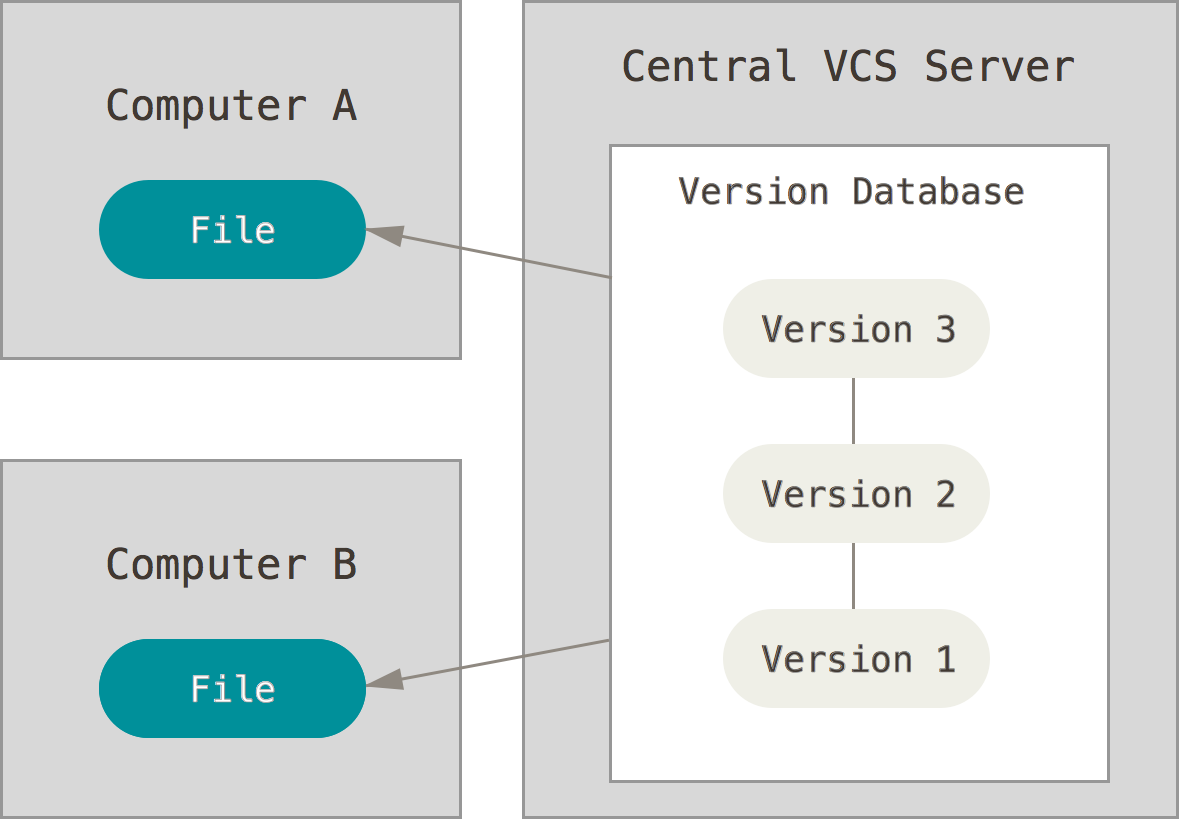
\includegraphics[width=0.8\textwidth]{VersionControlCentralized.png}
	\caption{Centralizētas VCS}
	\label{appfig:VersionControlCentralized}
\end{figure}

\begin{figure}[H]%!ht
	\centering
	\captionsetup{justification=centering}
	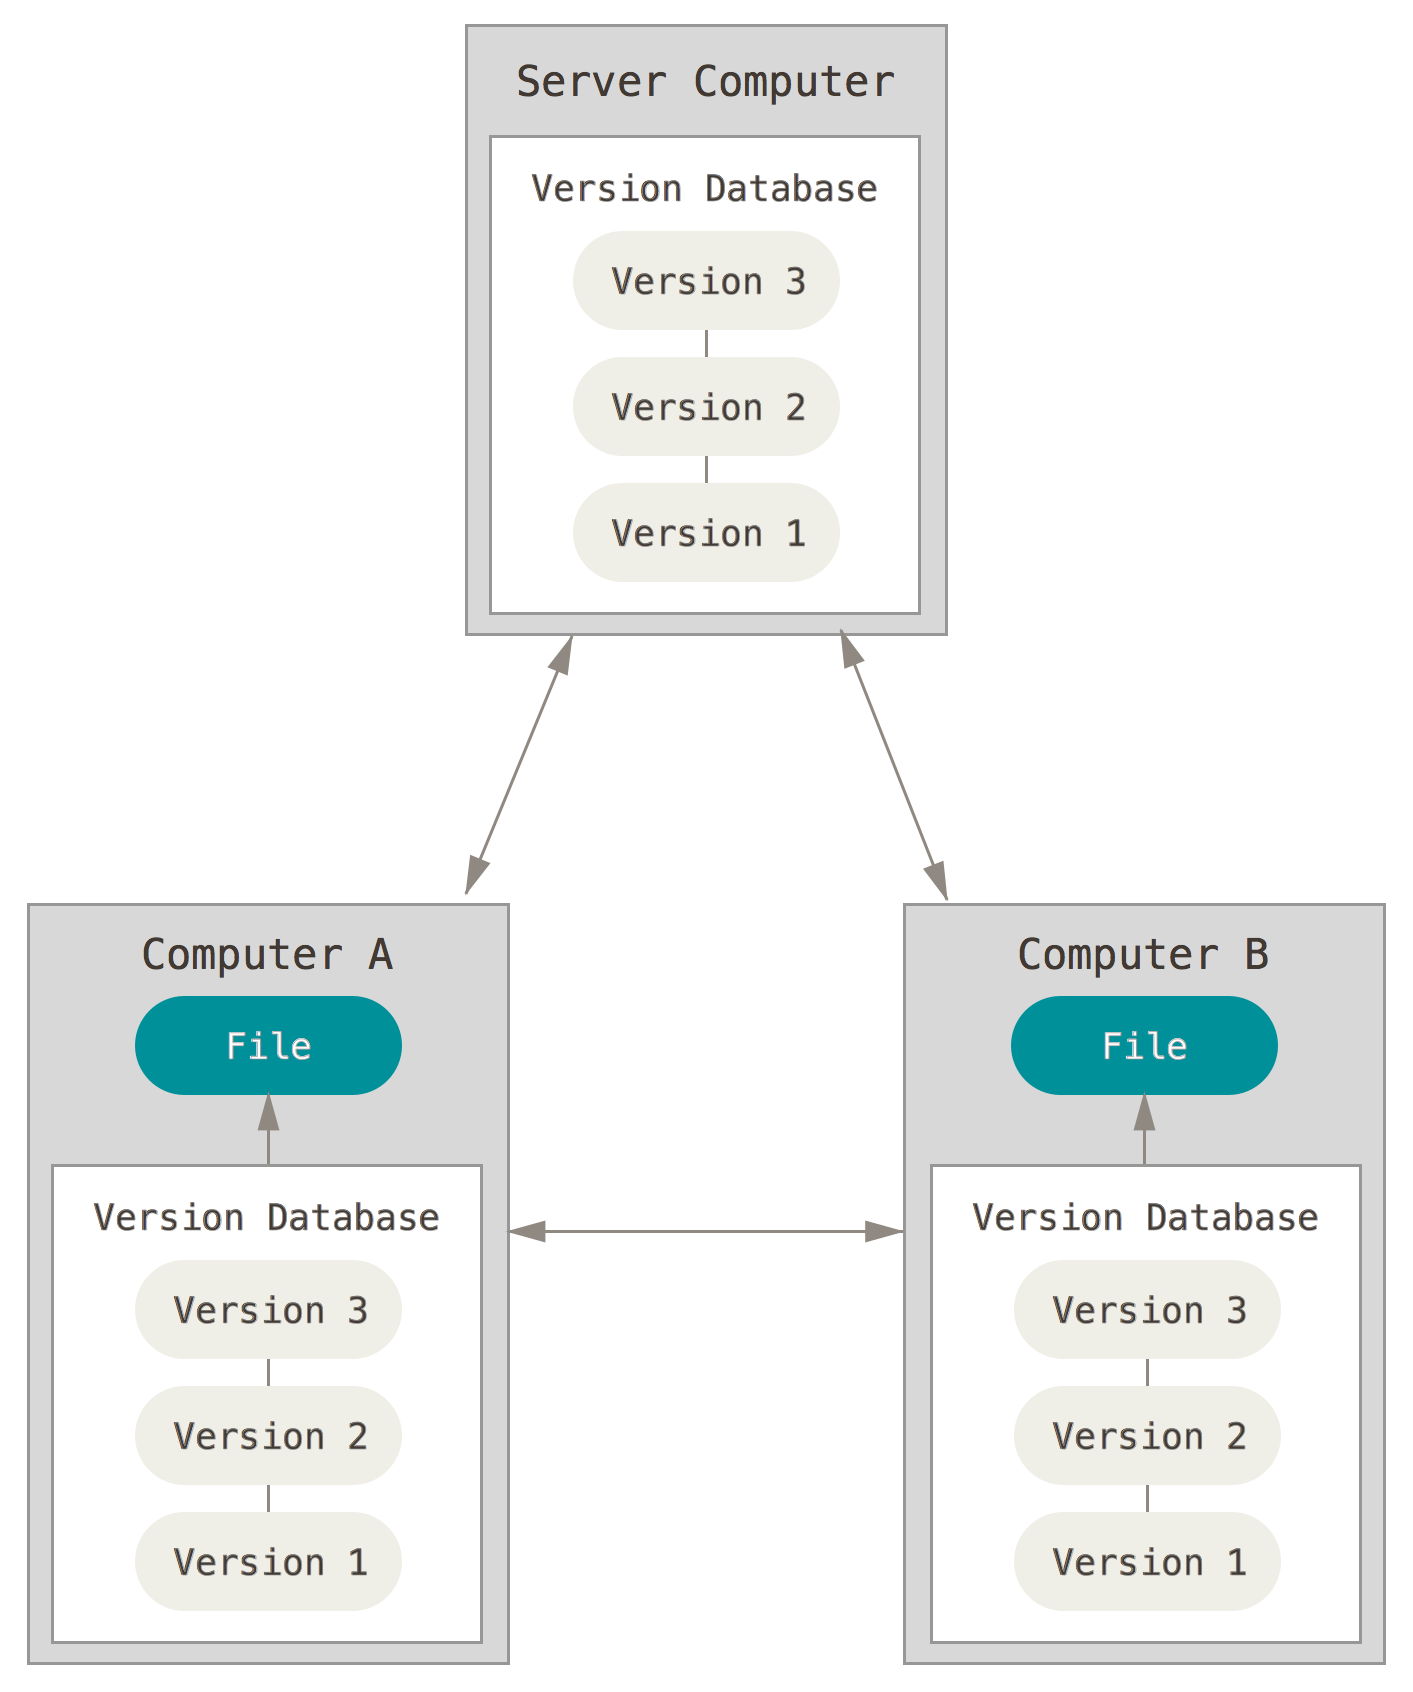
\includegraphics[width=1\textwidth]{VersionControlDistributed.png}
	\caption{Dalītas VCS}
	\label{appfig:VersionControlDistributed}
\end{figure}

\begin{figure}[H]%!ht
	\centering
	\captionsetup{justification=centering}
	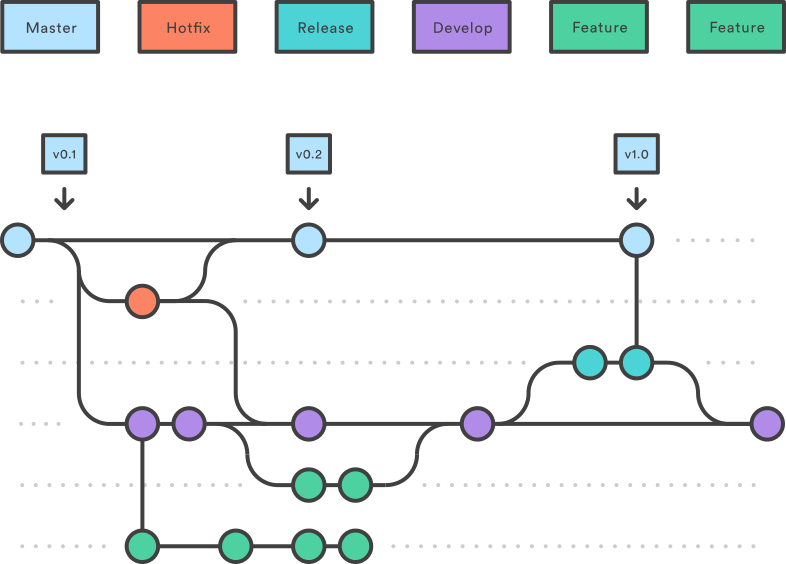
\includegraphics[width=1\textwidth]{WorkflowGitflow.png}
	\caption{Gitflow zarošanās stratēģijas attēlojums}
	\label{appfig:WorkflowGitflow}
\end{figure}

\begin{figure}[H]%!ht
	\centering
	\captionsetup{justification=centering}
	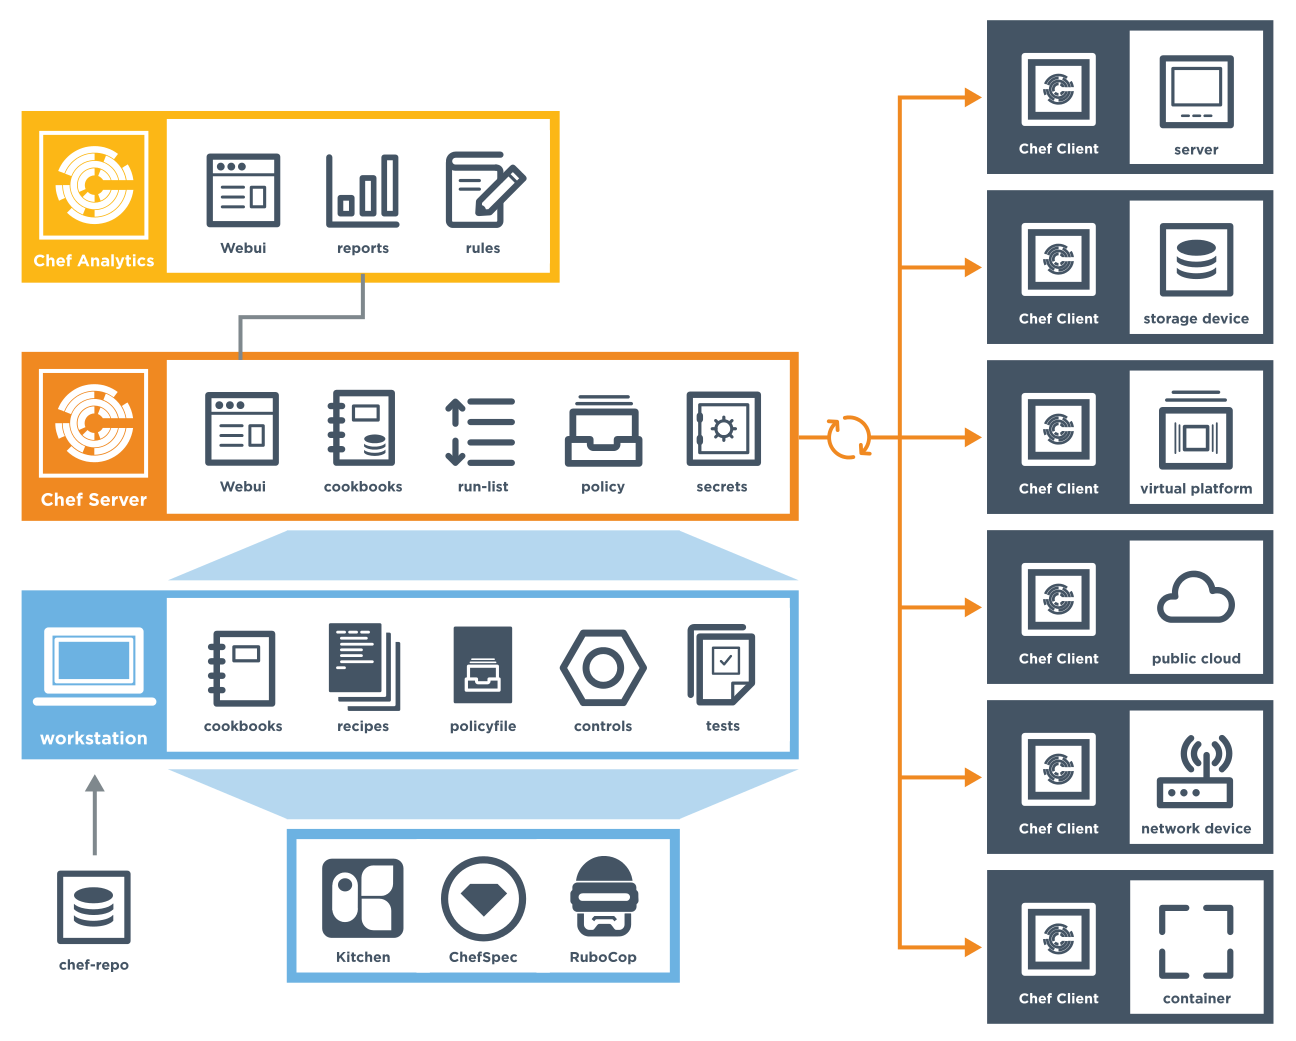
\includegraphics[width=1\textwidth]{ChefOverview.png}
	\caption{Chef komponentes}
	\label{appfig:ChefOverview}
\end{figure}

%==================================================================
\chapter{Pielikums}
\lstinputlisting[caption=Gemfile, label=appcode:gemfile]{code/Gemfile}
\lstinputlisting[caption=.gitignore, label=appcode:gitignore]{code/.gitignore}

\end{appendices}